% Figura Anexo I: la curva de PHILLIPS (1958) original: forma ajustada, corte y bucles cíclicos
\documentclass[tikz,border=3pt]{standalone}
\usepackage[T1]{fontenc}
\usepackage[utf8]{inputenc}
\usetikzlibrary{arrows.meta,calc}
\begin{document}
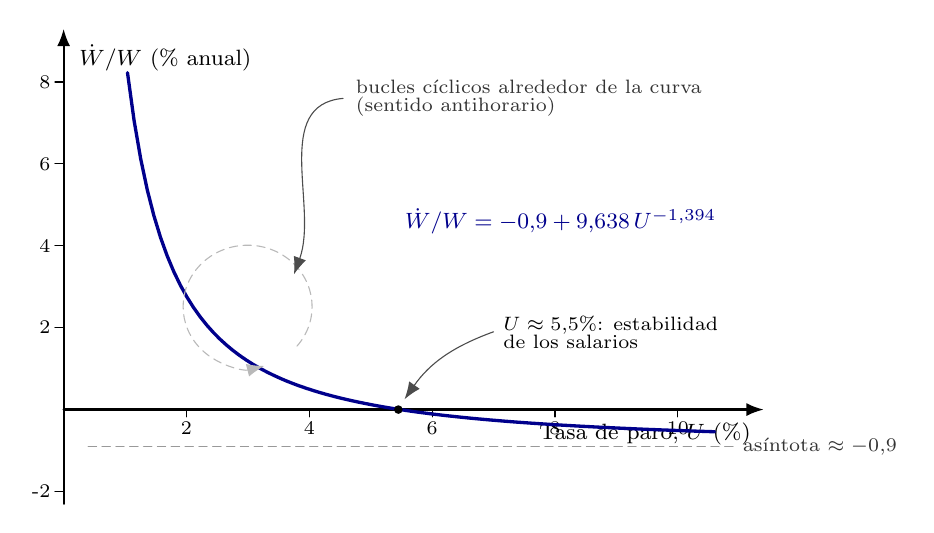
\begin{tikzpicture}[x=0.78cm, y=0.52cm, >={Latex[length=2.2mm]}, line cap=round, font=\footnotesize,
  eje/.style={->, thick},
  curva/.style={very thick},
  guia/.style={densely dashed, gray!80},
  pto/.style={circle, fill=black, inner sep=1.1pt}]
  % Ejes (el eje de abscisas en y=0; la zona negativa queda debajo)
  \draw[eje] (0,-2.3) -- (0,9.3) node[below right=2pt]{$\dot{W}/W$ (\% anual)};
  \draw[eje] (0,0) -- (11.4,0) node[below left=1pt]{Tasa de paro, $U$ (\%)};
  \foreach \u in {2,4,6,8,10} \draw (\u,0) -- (\u,-0.18) node[below, inner sep=1.5pt]{\scriptsize\u};
  \foreach \w in {-2,2,4,6,8} \draw (0,\w) -- (-0.14,\w) node[left, inner sep=1.5pt]{\scriptsize\w};
  % Curva ajustada de Phillips: w = -0,9 + 9,638 U^{-1,394}
  \draw[curva, blue!55!black] plot[domain=1.04:10.6, samples=90] (\x,{-0.9+9.638*exp(-1.394*ln(\x))});
  \node[blue!55!black, anchor=west] at (5.4,4.6) {$\dot{W}/W=-0{,}9+9{,}638\,U^{-1{,}394}$};
  % Asíntota inferior
  \draw[guia] (0.4,-0.9) -- (10.9,-0.9) node[right, gray!40!black]{\scriptsize asíntota $\approx -0{,}9$};
  % Corte con el eje
  \node[pto] at (5.45,0) {};
  \draw[<-, gray!60!black] (5.55,0.25) to[out=55,in=200] (7.0,1.9) node[right, black, align=left]{\scriptsize $U\approx 5{,}5\%$: estabilidad\\[-3pt]\scriptsize de los salarios};
  % Bucles cíclicos
  \draw[densely dashed, gray!55, ->] (3.8,1.55) arc[start angle=-40, end angle=285, x radius=1.05, y radius=1.5];
  \node[gray!40!black, align=left, anchor=west] at (4.6,7.6) {\scriptsize bucles cíclicos alrededor de la curva\\[-3pt]\scriptsize (sentido antihorario)};
  \draw[<-, gray!60!black] (3.75,3.3) to[out=70,in=185] (4.55,7.6);
\end{tikzpicture}
\end{document}
